\section{Lo strato data link}

\subsection{Progetto dello strato data link}
Lo strato data link si prende carico di diverse funzioni, fra cui:

\begin{enumerate}

\item{Definire un servizio di interfaccia per lo strato network};
\item{Gestire gli errori di trasmissione};
\item{Regolare il flusso di dati in modo che i dispositivi riceventi lenti non vengano sopraffatti dai trasmettitori veloci}.

\end{enumerate}

Per raggiungere questi obiettivi, lo strato prende i pacchetti che arrivano dallo strato network e li incapsula in \textbf{frame}, con uno \textit{header}, un \textit{corpo} e una \textit{coda}.

\begin{figure}[htbp]
\centering
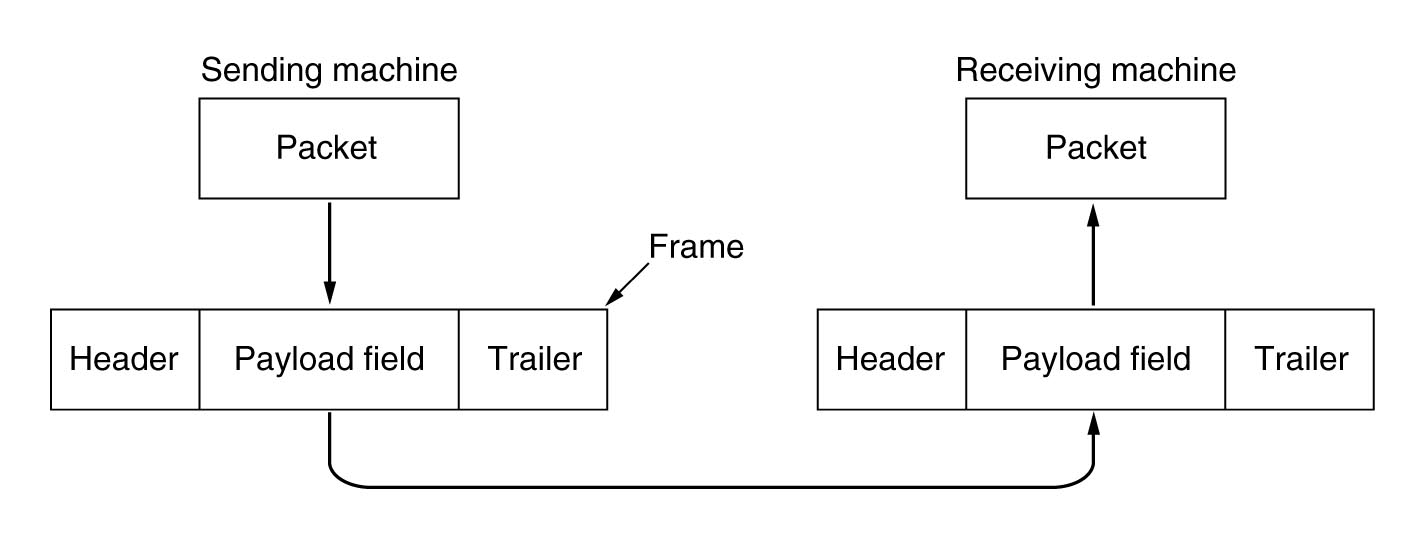
\includegraphics[scale=1]{images/package_frame.jpg}
\caption{Relazione fra pacchetti e frame}
\end{figure}

\subsubsection{Servizi}

La funzione dello strato data link consiste nel fornire servizi allo strato network. Il servizio principale è quello di trasferire dati dallo strato network della macchina sorgente allo strato network della macchina destinazione. Tre servizi che vengono comunemente forniti a questo livello sono:

\begin{enumerate}

\item{\textbf{Servizio unacknoledged senza connessione}: una macchina invia dei frame e non è necessaria una connessione dedicata e nemmeno una risposta e/o conferma del destinatario. Se il pacchetto viene perso non viene fatto nulla. Utile per canali con bassa percentuale di errori o per trasmissioni voce in cui il ritardo è peggiore di un errore};
\item{\textbf{Servizio acknoledged senza connessione}: anche qui non è necessaria una connessione, ma ogni frame è inviato singolarmente e si attende una conferma, entro un limite di tempo massimo, del destinatario. Se il limite è superato si reinvia il frame. Servizio utile per reti poco affidabili come le reti wireless};
\item{\textbf{Servizio acknoledged orientato alla connessione}: c'è bisogno di connessione tra le parti, poi si inizia a inviare. Ogni frame viene numerato. Tramite ACK viene garantita la ricezione e grazie alla numerazione si cerca di rilevarli nell'ordine esatto. Alla fine la comunicazione viene chiusa liberando i relativi buffer, variabili e risorse usate per mantenere la connessione}.

\end{enumerate}

\subsubsection{Suddivisione in frame}

Per servire lo strato network, lo strato data link deve usare a sua volta il servizio che gli è fornito dallo strato fisico, che ha come compito quello di prendere un flusso di bit e cercare di portarli a destinazione.
Il tipico approccio di questo strato consiste nel suddividere del flusso di bit in frame e calcolarne il cheksum, il quale viene ricalcolato dal destinatario che controlla la corrispondenza. In caso contrario si è verificato un errore e vengono presi i provvedimenti necessari. Un problema non banale è capire la suddivisione in frame, ovvero dove finisce o inizia un frame. Esistono 4 modi principali per farlo:

\begin{enumerate}

\item{Conteggio dei caratteri}
\item{Flag byte con byte stuffing}
\item{Flag di inizio e fine con bit stuffing}

\end{enumerate}

Il \textbf{primo metodo} banalmente inserisce nella testa un campo con il numero di caratteri di lunghezza del frame. Il problema principale è l'errore nel conteggio di caratteri durante la trasmissione che sfaserebbe tutto. Richiedere la ritrasmissione non è una soluzione perché il destinatario non capisce quanti caratteri deve saltare. Il \textbf{secondo metodo} aggira il problema inserendo un byte prima e dopo ogni frame, chiamato \textbf{flag byte}. Quindi in caso di perdita di sincronizzazione basterà cercare questo byte speciale. Un possibile problema è che all'interno dei dati ci sia un flag byte. Per risolverlo basta che la sorgente in tali casi inserisca un \textbf{byte di escape} (\textit{ESC}) subito prima di ogni occorrenza e la destinazione provvederà a toglierli (\textbf{destuffing}). Questa tecnica è chiamata \textbf{byte stuffing} (o \textbf{character stuffing}). Paradossalmente un ESC deve essere preceduto a sua volta da un ESC! Il problema di questo metodo è il legame con la decodifica dei caratteri con 8 bit che non è sempre vera. Il \textbf{terzo metodo} applica una tecnica simile alla precedente: ogni frame comincia e finisce con un gruppo speciale di bit, 01111110, in sostanza un flag byte. Ogni volta che lo strato Data link della sorgente incontra cinque 1 inserisce uno 0 subito dopo. Questa tecnica è detta \textbf{bit stuffing}. Il destinatario ovviamente incontrando cinque 1 e uno 0 non deve far altro che eliminare lo 0 per ottenere il messaggio originale.

\subsubsection{Controllo degli errori}
Per riuscire a rilevare banalmente errori nella trasmissione dei dati principalmente le cose da fare sono:\\ogni frame deve avere un numero di sequenza in modo che la destinazione accetta solo i frame che non ha già ricevuto, la sorgente ha un timer utile per quando attende che l'ACK ritorni dal destinatario in modo da non fare attesa infinita. Se non riceve ACK in un tempo limite stabilito dal protocollo il messaggio viene reinviato.

\subsubsection{Controllo del flusso}
Esistono principalmente 2 tecniche per la gestione del flusso (evitando così sovraccaricamenti del desinatario):
\begin{enumerate}
\item{Tramite Feedback: la destinazione manda alla sorgente informazioni per darle il permesso di inviare altri dati o comunque per informarla dello stato in cui si trova.}
\item{Tramite limitazione di velocità: il protocollo contiene al suo interno un meccanismo che limita la velocità della sorgente senza utilizzo di feedback.}
\end{enumerate}

\subsection{Rilevazione e correzione degli errori}
\subsubsection{Codici per la correzione degli errori}
Esistono principalmente 2 tipi di decodifica: a semplice rilevazione di errori e a correzione di errore. Entrambe consistono nell'aggiunta di informazioni ridondanti per rilevare e nel secondo caso correggere gli errori. Le 2 tecniche vanno applicate ovviamente in ambiti differenti, la prima più indicata per trasmissioni veloci tipo con fibra, mentre la seconda per trasmissioni più rumorose come quelle wireless. \\
Come avviene l'identificazione di un errore: in primo luogo indichiamo con n la lunghezza di una \textbf{codeword} formata da m bit per il frame e r per il controllo (n = m+r). Confrontando ora 2 codeword di lunghezza uguale facendo semplicemente lo XOR troviamo tutti 0 se le parole coincidono oppure alcuni 1. La quantità di 1 presenti corrisponde alla \textbf{distanza di Hamming}. Una distanza di Hamming \textit{d} rappresenta il numero di errori per convertire una sequenza nell'altra. Essendo che non tutte le possibili \(2^m\) codeword sono accettabili, un modo per intuire la codeword esatta è enumerare tutte le possibili codeword e scegliere quelle con distanza di Hamming minima. In base a alla distanza d+1 della codifica si riescono a trovare d errori. Mentre per correggerne d ci vorrebbe una codifica con distanza 2d + 1. Un esempio lo è il bit di parità.

\subsubsection*{Codifica di Hamming}
Vengono inseriti nella sequenza di bit da inviare bit di parità posti nelle posizioni che sono una potenza di 2. Questi bit di parità sono legati ad alcuni bit di dati con la seguente regola: il bit di dati k-esimo è controllato da quei bit la cui somma forma k. Per esempio k = 11 = 1 + 2 + 8, allora il primo, secondo e ottavo bit sono quelli di parità per k. Quindi se troviamo errori di inversione nei bit 1,2 e 8 allora l'11 è invertito. Questa codifica corregge solo errori singoli. Esiste un trucco nell'invio di dati per correggere gli errori improvvisi, detti \textbf{burst}, che è quello di inviare le varie codeword sotto forma matriciale inviando i dati colonna per colonna in modo che gli errori burst siano solamente singoli bit per ogni riga e si sa che tramite hamming si possono correggere.

\subsubsection{Codifiche a rilevazione d'errore}
\subsubsection*{CRC \textit{(Cyclic Redundance Check)}}
L'idea di base è quella di trattare le sequenze di bit come coefficiente di polinomi. Si applica per cui l'aritmetica dei polinomi in modulo 2. Quindi addizioni e sottrazioni sono fatte con lo XOR. Un divisore sta in un dividendo se ha gli stessi bit. Quando si utilizza CRC la sorgente e la destinazione devono accordarsi su un \textbf{polinomio generatore} \textit{G(x)} che deve avere come primo e ultimo bit 1. Il frame da controllare, che corrisponde al polinomio \textit{M(x)}, deve essere di ordine maggiorne di G(x). L'idea è quella di aggiungere un checksum alla fine del frame in modo che il polinomio rappresentato dal frame col checksum sia divisibile per G(x). Per cui la destinazione riceve il polinomio e prova a dividerlo per G(x). Se c'è resto allora c'è errore.\\
Il calcolo del checksum avviene così:
\begin{enumerate}
\item{Posto r il grado di G(x), aggiungere r zeri alla fine del frame, così da avere m+r bit e corrisponde al polinomio \( x^r M(x)\)}
\item{Dividere la sequenza corrispondente a \( x^r M(x)\) per quella di G(x) usando la divisione modulo 2.}
\item{Sottrarre il resto, al massimo r bit, dalla sequenza corrispondente \( x^r M(x)\), sottrazione in modulo 2. Il risultato sarà \textit{T(x)}}
\end{enumerate}

\subsection{Protocolli Data Link elementari}
\subsubsection{Protocollo stop-and-wait}
Protocollo molto semplice per il controllo del flusso e si può utilizzare in canali simplex o half duplex. Quando il mittente invia un blocco aspetta che il ricevente invii una conferma (ACK). Lo svantaggio è l'attesa della risposta, ma in compenso non c'è bisogno di regolare la velocità. Gli errori possibili ora sono 2:
\begin{enumerate}
\item{Sul frame: ovvero non arriva mai a destinazione e quindi il mittente aspetta all'infinito. C'è bisogno di un timeout come detto precedentemente.}
\item{Sul ACK: la conferma non arriva al mittente, il quale al termine del time out reinvia il pacchetto. Al destinatario arriva 2 volte ma grazie al numero di pacchetto (vedi su) il pacchetto non viene preso in considerazione.}
\end{enumerate}
\subsection{Protocolli sliding window}
Un protocollo per il controllo di flusso sicuramente più efficiente di quello appena presentato. Un dettaglio sicuramente a suo favore è l'utilizzo della tecnica di \textbf{piggybacking}, che consiste nello sfruttare un messaggio del destinatario al mittente come 'passaggio' per il messaggio di conferma ACK, in modo da non perdere tempo e sfruttare maggiormente il canale di comunicazione. Il campo \textit{ack} è posto nella testa del frame. Sorge il problema di quando fare piggybacking, un attesa troppo lunga può rendere vano il tutto perché il mittente fa un reinvio del frame. Quindi se il pacchetto arriva velocemente viene fatto piggybacking dell'ACK altrimenti si invia l'ACK separatamente. L'essenza del protocollo è che ogni partecipante alla comunicazione deve tener sotto controllo 2 finestre: quella dei frame in entrata e quella dei frame in uscita. Ogni frame in uscita contiene un numero di sequenza e il destinatario deve tener traccia di questi per la ricezione mentre il mittente per l'invio. 
\begin{figure}[htbp]
\centering
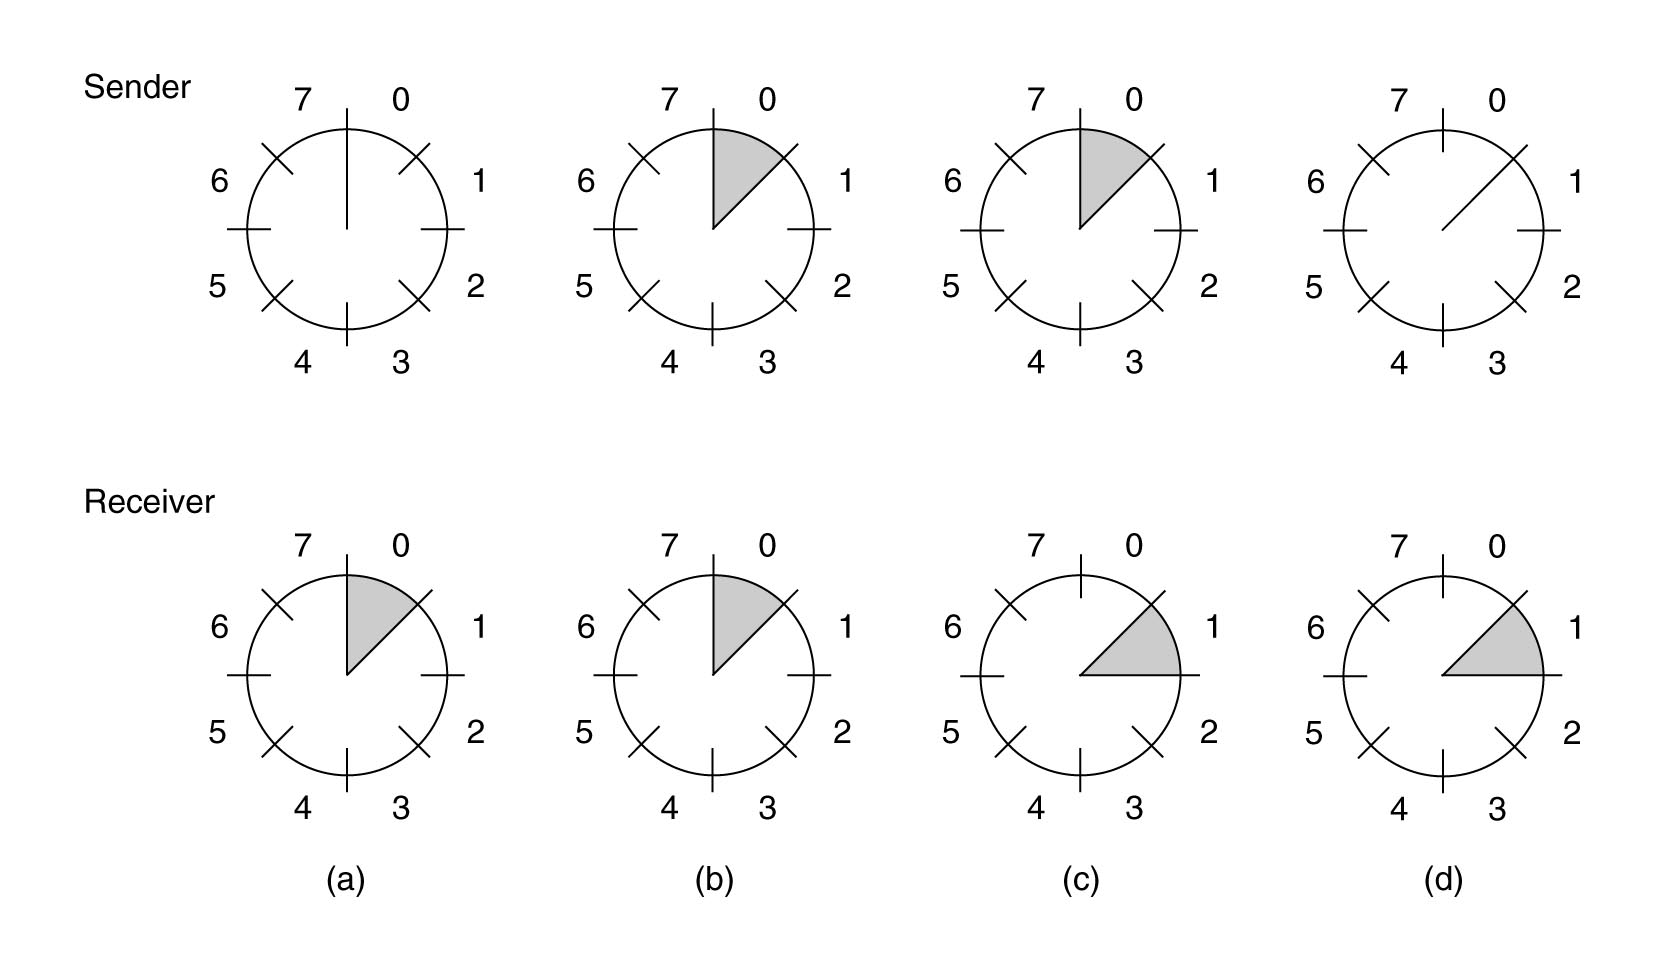
\includegraphics[scale=0.7]{images/sw.jpg}
\caption{Esempio sliding window: (a) Inizialmente, (b) Dopo l'invio del frame 0, (c) Dopo la sua ricezione, (d) Dopo l'invio dell'ACK.}
\end{figure}

\subsubsection{Protocollo sliding window a 1 bit}
La finestra di controllo ha dimensione 1 e viene utilizzato il metodo stp-and-wait. Quando il mittente invia un frame resta nella finestra finché non viene ricevuto l'ACK corrispondente prima di aggiornare la finestra. I frame inviati sono numerati con 1 o 0. Quando il destinatario riceve il frame controlla che il numero sia uguale a quello che aspettava, se si invia l'ACK. Se l'ACK contiene il numero che la sorgente si aspettava allora continua a inviare un nuovo pacchetto altrimenti reinvia quello segnato nel buffer. Si può utilizzare anche la tecnica \textbf{pipelining}, ovvero vengono inviati più frame contemporaneamente prima di entrare in attesa. Il destinatario aggiorna la finestra non appena riceve il frame e invia l'ACK. Esistono 2 approcci per contro i problemi di trasmissione durante il pipelining: uno chiamato \textbf{go back n} che semplicemente scarta tutti i frame dopo quello danneggiato, l'altra è la \textbf{ripetizione selettiva} nel quale vengono tenuti i frame buoni e non scartati e vengono messi in un buffer. Quando la sorgente va in timeout solo quello senza ACK viene rispedito. La destinazione quando trova un errore non sta "ferma", ma invia un NAK in modo da stimolare la ritrasmissione prima del timeout.

\subsubsection{Protocollo che usa go back n}
Qui la finestra di invio ha dimensione \(>\) 1 mentre quella di ricezione è uguale a 1. I pacchetti arrivano uno alla volta e su di essi viene fatto il checksum, se si trovano errori vengono segnalati alla sorgente indicando il numero del pacchetto danneggiato, per questo la finestra sorgente deve essere capiente. Se la finestra sorgente si riempie prima che il timer scatti, la pipeline viene svuotata. Le conferme vengono sempre mandate in piggybacking. La destinazione nel frattempo scarta i pacchetti successivi a quello avente l'errore. Questo approccio può far perdere molta banda se la frequenza degli errori è alta.
\begin{figure}[htbp]
\centering
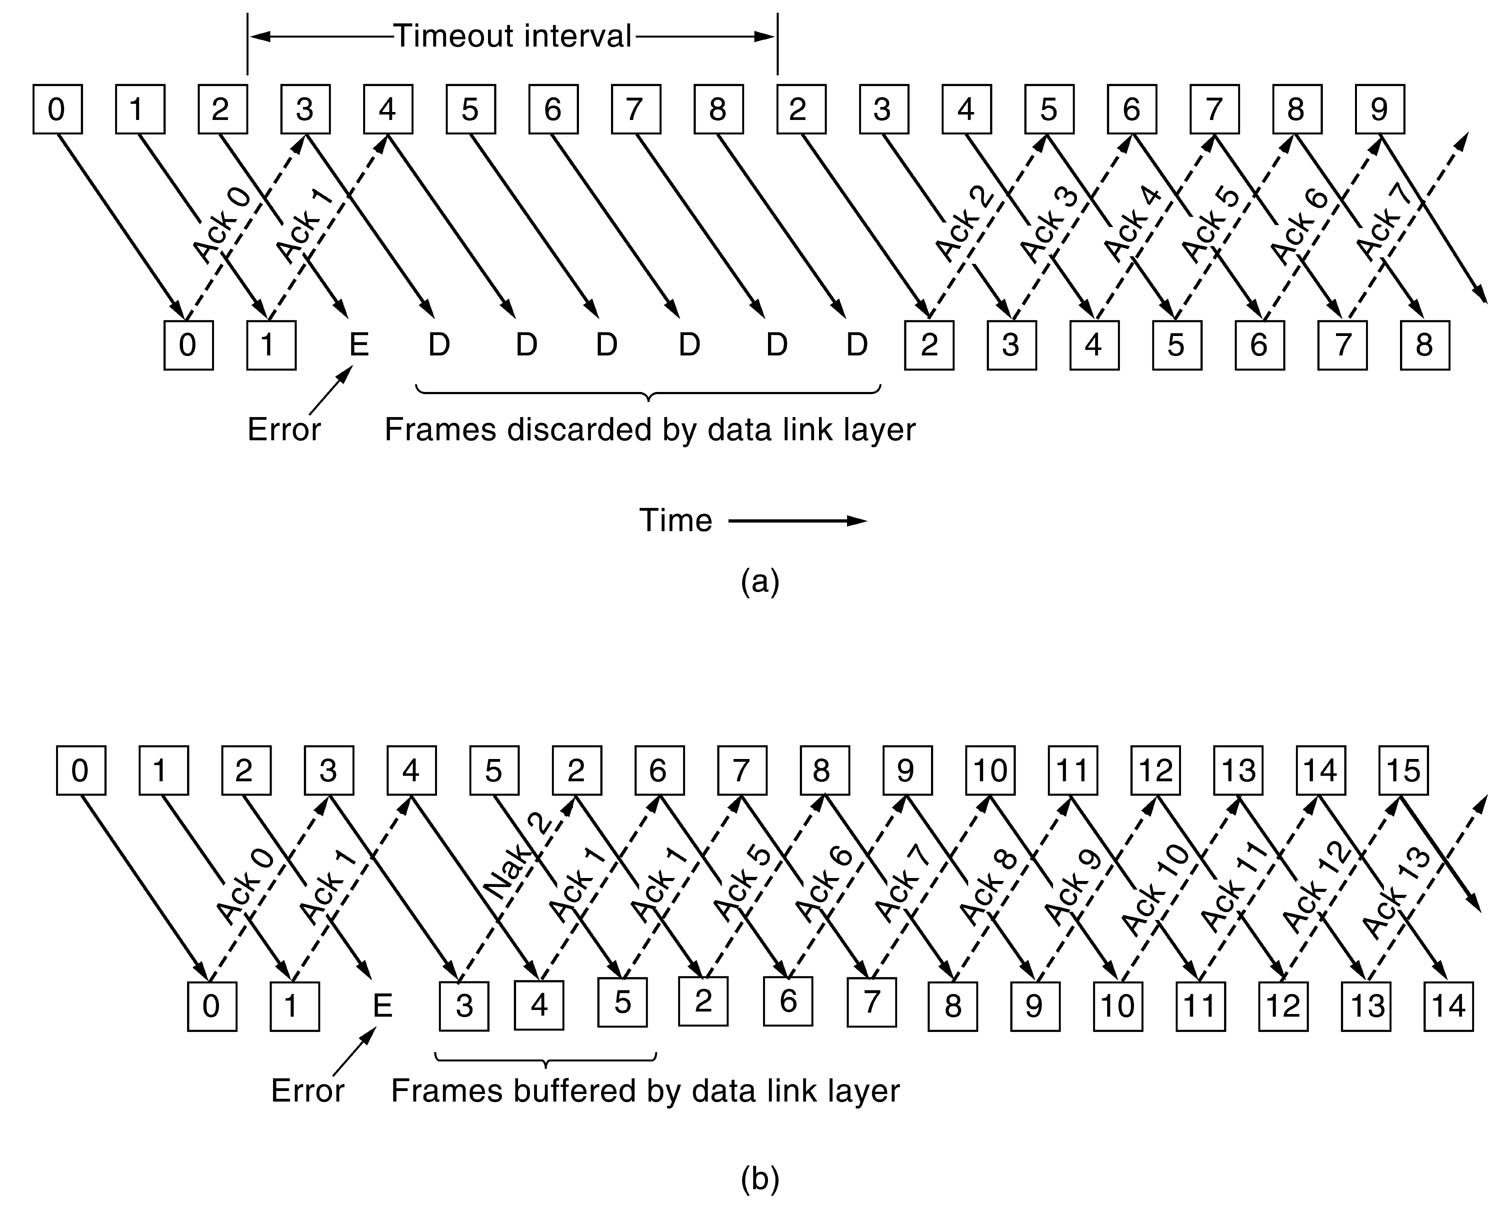
\includegraphics[scale=0.7]{images/gobackn.jpg}
\caption{Esempio sliding window con \textit{go back n}: effetti del pipelining.}
\end{figure}

\subsubsection{Protocollo che usa ripetizione selettiva \textit{(selective repeat)}}
In questo caso il buffer della destinazione deve essere più capiente. Nel caso di errori viene inviato alla sorgente un NACK (\textit{Not ACK}) indicandone il pacchetto. Finché il pacchetto errato non arriva nuovamente dalla sorgente i pacchetti successivi vengono posti nel buffer. Una volta arrivato tutto viene passato allo strato Network. \textit{Nota}: la sorgente dispone di timer per cui se non arrivasse il NACK il pacchetto viene reinviato comunque.

\subsection{Protocolli data link}
\subsubsection{HDLC (High-level Data Link Control)}
Deriva dal protocollo SDLC della IBM con le varianti LAP e LAPB. E' un protocollo orientato ai bit e usa il bit stuffing. La struttura dei frame di questo protocollo è:
\begin{figure}[htbp]
\centering
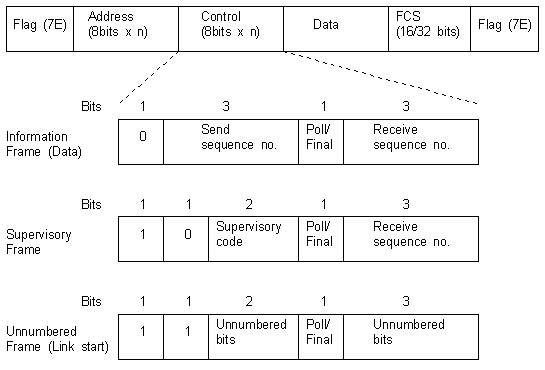
\includegraphics[scale=0.8]{images/hdlc.png}
\caption{Struttura frame HDLC}
\end{figure}
FCS indica la parte di checksum eseguita con CRC, Flag(7E) è il flag 01111110, mentre il Control con le Sliding Window e determina 3 tipi di frame:
\begin{enumerate}
\item{\textbf{Information}: formato da uno 0 seguito dal numero del frame. Poi p/f è utile per le conversazioni multiple e infine ci sono gli ACK (piggybacking sul frame successivo).}
\item{\textbf{Supervisory}: formato da uno 10 seguito dal campo type che può assumere 4 valori:
\begin{enumerate}
\item {Type 0: Frame ACK (Receive Ready)}
\item {Type 1: Frame NACK (Reject)}
\item {Type 2: Canale congestionato (Receive NOT Ready)}
\item {Type 3: NACK selettivo (Selected Reject)}
\end{enumerate}
Il resto come il precedente.}
\item{\textbf{Unnumbered}: formato da uno 11. Viene usato nel caso di perdita di frame.}
\end{enumerate}

I principalei comandi sono:
\begin{itemize}
\item{DISC: blocca la connessione}
\item{SNRM: nuova macchina on-line}
\item{SAMB: crea una connessione bilanciata}
\item{FRMR: rifiuta un frame di controllo}
\end{itemize}

\subsubsection{PPP \textit{(Point-to-Point Protocol)}}
Usato nei collegamenti punto a punto tra router e utente, ovvero in internet. Tra le varie funzioni di PPP troviamo: rilevazione degli errori, supporto per più protocolli, possibilità di negoziazione IP, possibilità di effettuare autenticazione. Tra le caratteristiche di questo protocollo meritano menzione:
\begin{enumerate}
\item{Metodo di framing che permettere di limitare i vari frame in modo non ambiguo e il formato del frame permette la rilevazione degli errori}
\item{Protoccolo di collegamento per gestire la connessione, i test, le negoziazioni e la gestione pulita della disconnessione. (LCP)}
\item{Modalità per negoziare le opzioni relative allo strato Network.}
\end{enumerate}
Utilizza 2 protocolli speciali:
\begin{enumerate}
\item{\textbf{LCP}\textit{(Link Control Protocol)}: insieme di comandi per la gestione del flusso e della comunicazione}
\item{\textbf{NCP}\textit{(Network Control Protocol)}: si occupa del dialogo con lo strato 3}
\end{enumerate}
La differenza più importante dall'HDLC è l'utilizo del byte stuffing.
Il frame PPP è così composto:
\begin{figure}[htbp]
\centering
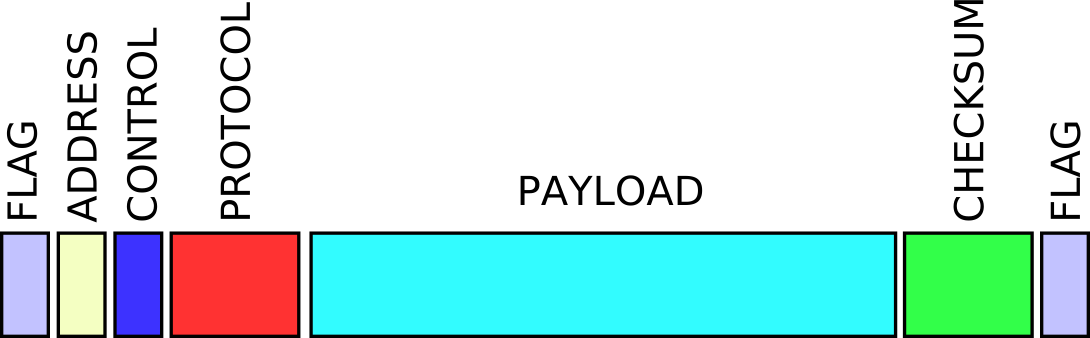
\includegraphics[scale=0.3]{images/ppp.png}
\caption{Struttura frame PPP}
\end{figure}
\begin{itemize}
\item{\textbf{FLAG}: flag byte tipico 01111110}
\item{\textbf{Address}: non viene usato, tutti 1}
\item{\textbf{Control}: posto per default a 00000011, ovvero niente controllo}
\item{\textbf{Protocol}: segnala il tipo di pacchetto che si invia}
\item{\textbf{Payload}: campo dati}
\item{\textbf{Checksum}: usa CRC}
\item{\textbf{FLAG}: di nuovo flag byte tipico}
\end{itemize}